\documentclass[../sherrill-Mix_thesis.tex]{subfiles}
\begin{document}
\graphicspath{{im/}{rnaSeq/im/}}


\newcommand{\nReads}{1,161,705,678}
\newcommand{\nHuman}{1,021,207,853}
\newcommand{\nHIV}{24,783,844}
\newcommand{\nHIVFrag}{12,689,879}
\newcommand{\nIntegrations}{147,281}


\chapter{Gene activity in primary T cells infected with \hivEight{}: intron retention and induction of distinctive genomic repeats}
\label{chapRnaSeq}

\textBox{This chapter is under review as:\\
	\citeBox{Sherrill-MixUnderReview}

	KE Ocwieja performed the infections and sequencing. I analyzed the data. KE Ocwieja, FD Bushman and I planned the overall study. I produced the figures. FD Bushman and I wrote the paper. 
%	Additional files are available at \url{http://www.retrovirology.com/content/10/1/90/additional}
}

\section{Abstract}
	Background: HIV infection has been reported to alter cellular gene activity, but published studies have commonly assayed transformed cell lines and lab-adapted HIV strains, yielding inconsistent results. Here we carried out a deep RNA-Seq analysis of primary human T cells infected with the low passage HIV isolate \hivEight{}. 

	Results: Seventeen percent of cellular genes showed altered activity 48 hours after infection. In a meta-analysis including four other studies, our data differed from studies of transcription after HIV infection of cell lines but showed more parallels with infections of primary cells. We found a global trend toward retention of introns after infection, suggestive of a novel cellular response to infection. \hivEight{} infection was also associated with activation of human endogenous retroviruses (HERVs) and several retrotransposons, of interest as possible novel antigens that could serve as vaccine targets. The most highly activated group of HERVs was a subset of the ERV-9, a group not reported previously to be induced by HIV. Analysis showed that activation was associated with a particular variant of an ERV-9 long terminal repeat that contains an indel near the U3-R border. These data also allowed quantification of \textgreater{}70 splice forms of the \hivEight{} RNA and specified the main types of chimeric \hivEight{}-host RNAs. Comparison to \nIntegrations{} integration site sequences from the same infected cells allowed quantification of authentic versus artifactual chimeric reads (0.1\% of the total), showing that \fivePrime{} read-in, splicing out of \hivEight{} from the D4 donor and \threePrime{} read-through were the most common \hivEight{}-host cell chimeric RNA forms. 

	Conclusions: Analysis of RNA abundance after infection of primary T cells with the low passage \hivEight{} isolate disclosed multiple novel features of HIV-host interactions, notably intron retention and induction of transcription of distinctive retrotransposons and endogenous retroviruses.

\section{Background}
	HIV replication requires integration of a cDNA copy of the viral RNA genome into cellular chromosomes, followed by transcription and splicing to yield viral mRNA. Alternative splicing allows the small 9.1 kb HIV genome to generate at least 108 mRNA transcripts encoding at least 9 proteins and polyproteins  \citep{Wain-Hobson1985,Arya1985,Schwartz1990,Purcell1993,Stoltzfus2009,Ocwieja2012}. During replication, HIV also reprograms cellular transcription and splicing. For example, the virus-encoded Vpr protein arrests the cell cycle \citep{He1995,Jowett1995,Rogel1995,Goh1998} and the viral Tat protein binds to P-TEFb and alters transcript at the HIV promoter and some cellular promoters \citep{Marciniak1991,Wei1998,Kanazawa2000,Barboric2007,OBrien2010,Muniz2010}. 

	Multiple studies suggest that cells detect HIV infection and respond by inducing inter\-feron-regulated, apoptotic and stress response pathways \citep{Corbeil2001,Woelk2004,Hyrcza2007,Wu2008,Smith2010,Chang2011,Imbeault2012,Mohammadi2013,Peng2014}. Several studies have also suggested that HIV infection disrupts normal cellular splicing pathways \citep{Dowling2008,Peng2014}. However, results have varied with many experimental parameters, including target cell type, HIV isolate and the duration of infection. Many of the published studies focused on infections with lab-adapted HIV strains in transformed cell lines \citep{Corbeil2001,Mitchell2003,delaFuente2002,Chang2011,Lefebvre2011,Peng2014}, and so results may not be fully reflective of infections in patients.

	In this study, we sought to generate data more resembling HIV replication in patients by analyzing transcriptional responses after infection of primary T cells with \hivEight{}, a low passage patient isolate \citep{Collman1992}.  This represents a continuation of a long term effort to understand HIV-host cell interactions at the transcriptional level that began with analysis of transcription by \hivEight{} in primary T cells using Pacific Biosciences long read single molecule sequencing \citep{Ocwieja2012}. Our strategy here was to analyze a single time after infection in depth, analyzing over 1 billion sequence reads from \hivEight{} infected and uninfected host cells. These data were then combined with \nIntegrations{} unique integration site sequences from the same infections and the Pacific Biosciences data on \hivEight{} transcription to 1) elucidate effects of HIV infection on host cell mRNA abundances and splicing, 2) characterize viral message structure in detail and 3) probe the nature of the chimeras formed between host cell and viral RNAs.  

\section{Methods}
	\subsection{Cell culture and viral infections}
		\hivEight{} stocks were generated by the University of Pennsylvania Center for Aids Research. 293T cells were transfected with a plasmid encoding an \hivEight{} provirus, and harvested virus was passaged in SupT1 cells once. Viral stocks were quantified by measuring p24 antigen content.  Primary \cdFour{} T cells were isolated by the University of Pennsylvania Center for AIDS research Immunology Core from apheresis product from a single healthy male donor (ND365) using the RosetteSep Human \cdFour{} T Cell Enrichment Cocktail (StemCell Technologies).

		T cells were stimulated for 3 days at $0.5 \times 10^6$ cells per milliliter in R10 media (RPMI 1640 with GlutaMAX (Invitrogen) supplemented with 10\% FBS (Sigma-Aldrich) with 100 units U/mL recombinant IL2 (Novartis) + 5$\mu$g/mL PHA-L (Sigma-Aldrich)).  Cells were infected in triplicate and mock infections were performed in duplicate.  For each infection, $6.6 \times 10^6$ cells were mixed with 1.32 $\mu$g \hivEight{} in a total volume of 2.25 mL.  Infection mixtures was split into three wells of a 6 well plate for spinoculation at 1200 g for 2 hr at 37\degree{}C.  Cells were incubated an additional 2 hr at 37\degree{}C.  Cells were then pooled into flasks and volume was increased to a total of 12 mL.  Spreading infection was allowed to proceed 48 hr at 37\degree{}C, after which cells were harvested.  $1 \times 10^6$ cells were harvested for flow cytometry, and $6 \times 10^6$ cells were pelleted following two washes in PBS for nucleic acid extraction.  Genomic DNA and total RNA were isolated from $6 \times 10^6$ T cells per infection using the AllPrep DNA/RNA Mini Kit (Qiagen) with Qiashredder columns (Qiagen) for homogenization according to the manufacturer's instructions.  DNA was eluted in 140 $\mu$L elution buffer.   RNA samples were treated with DNase prior to elution in 40 $\mu$L water.
		
	\subsection{Analysis of \hivEight{} integration sites in primary T cells}
		Integration site sequences were determined for DNA fractions from the above infections after ligation mediated PCR \citep{Berry2014}. A total of \nIntegrations{} unique integration site sequences were determined. An analysis of integration site distributions for these samples was reported in \citet{Berry2014}. 

	\subsection{mRNA sequencing}
		Messenger RNA was isolated and amplified from purified total cellular RNA (3 $\mu$L or approximately 9 $\mu$g from each uninfected sample, 25 $\mu$L or approximately 3 $\mu$g from each infected sample) using the Illumina TruSeq RNA sample preparation kit according to manufacturer's protocol.  SuperScript III (Invitrogen) was used for reverse transcription. Each sample was tagged with a separate barcode and sequenced on an Illumina HiSeq 2000 using 100-bp paired-end chemistry. 

	\subsection{Flow cytometry}
		To assess percent infected cells, $1 \times 10^6$ cells per infection were stained for flow cytometry.  All staining incubations were at room temperature.  Cells were first washed in PBS and then twice in FACS wash buffer (PBS, 2.5\% FBS, 2 mM EDTA).  Cells were fixed and permeabilized with CytoFix/CytoPerm (BD) for 20 minutes and washed with Perm-Wash Buffer (BD) before staining with anti-HIV-Gag-PE (Beckman Coulter) for 60 min.  Finally cells were washed in FACS wash buffer and resuspended in 3\% PFA.  Samples were run on a LSRII (BD) and analyzed with FlowJo 8.8.6 (Treestar). Cells were gated as follows: lymphocytes (SSC-A by FSC-A), then singlets (FSC-A by FSC-H), then by Gag expression (FSC-A by Gag). 

	\subsection{Analysis}
		Reads were aligned to the human genome using a combination of BLAT \citep{Kent2002} and Bowtie \citep{Langmead2009} through the Rum pipeline \citep{Grant2011}.  Estimates of fragments per kilobase of transcript per million mapped reads and changes in expression for cellular genes were calculated by Cufflinks \citep{Trapnell2010}. Reads found to contain sequence similar to the HIV genome using a suffix tree algorithm were aligned against the \hivEight{} genome using BLAT \citep{Kent2002}. All statistical analyses were performed in R 3.1.2 \cite{RCoreTeam2012}. RNA-Seq reads from \citet{Chang2011} were downloaded from the Sequence Read Archive (SRP013224) and aligned using the Rum pipeline.

		Gene lists were obtained from the supplementary materials of four other studies of differential gene expression during HIV infection \citep{Li2009,Imbeault2012,Lefebvre2011,Chang2011}. We called genes differentially expressed in \citet{Li2009} if they had a reported $p<0.01$ or in \citet{Lefebvre2011}, \citet{Chang2011} and \citet{Imbeault2012} if they had an adjusted $p<0.05$. We called genes as differentially expressed in our own study if the adjusted $p<0.01$. For the comparison of differentially expressed genes regardless of direction in figure \ref{figGenes} (below the diagonal), it was unclear exactly how many genes were studied in each study so we assumed a background of the 14,192 genes (the number of genes which could be tested for significance in our data). 
		
		We obtained transcriptional profiles comparing immune cell subsets from the Molecular Signatures Database \citep{Subramanian2005}. MSigDB set names from the MSigDB used in Figure \ref{figMsig}A were GSE10325 LUPUS CD4 TCELL VS LUPUS BCELL, GSE10325 CD4 TCELL VS MYELOID, GSE10325 CD4 TCELL VS BCELL, GSE10325 LUPUS CD4 TCELL VS LUPUS MYELOID, GSE3982 MEMORY CD4 TCELL VS TH1, GSE22886 CD4 TCELL VS BCELL NAIVE, GSE11057 CD4 CENT MEM VS PBMC, GSE11057 CD4 EFF MEM VS PBMC, GSE3982 MEMORY CD4 TCELL VS TH2 and GSE11057 PBMC VS MEM CD4 TCELL and in Figure \ref{figMsig}B were GSE36476 CTRL VS TSST ACT 72H MEMORY CD4 TCELL OLD, GSE10325 CD4 TCELL VS LUPUS CD4 TCELL, GSE22886 NAIVE CD4 TCELL VS 12H ACT TH1, GSE3982 CENT MEMORY CD4 TCELL VS TH1, GSE17974 CTRL VS ACT IL4 AND ANTI IL12 48H CD4 TCELL, GSE24634 IL4 VS CTRL TREATED NAIVE CD4 TCELL DAY5, GSE24634 NAIVE CD4 TCELL VS DAY10 IL4 CONV TREG, GSE1460 CD4 THYMOCYTE VS THYMIC STROMAL CELL and GSE1460 INTRATHYMIC T PROGENITOR VS NAIVE CD4 TCELL ADULT BLOOD. 
		
		We downloaded the RepeatMasker track from the UCSC genome browser \citep{Kent2002a} and used the SAMtools library \citep{Li2009a} to assign reads to the repeat regions. HERV-K age estimates were obtained from the supplementary materials of \citet{Subramanian2011}.

		 We used a Bayesian estimate of the ratio of expression in uninfected and HIV infected samples to account for sampling effort and differing expression in genomic regions. We modeled the observed counts as a binomial distribution with a flat beta prior ($\alpha=1,\beta=1$) separately for uninfected and infected samples. We then Monte Carlo sampled the two posterior distribution to estimate the posterior distribution of the ratio. For introns, the number of binomial successes was set to the number of reads mapped to the intron and the number of trials was the total number of reads observed in the genes overlapping that intron. For repeat regions, the number of binomial successes was set to the number of reads mapped to that region and the number of trials was the total number of reads mapped to the human genome.

		To estimate determinants of LTR12C expression, we fit a logistic regression for which LTR12C increased in expression with \hivEight{} infection (95\% Bayesian credible interval \textgreater{}1) on to characteristics of the LTR12C regions. We extracted all the LTR12C regions from the human genome and determined the U3-R boundary using a ends free alignment of the previously reported U3-R border \citep{LaMantia1991,LaMantia1992,Plant2001,Ling2002,Yu2005} against the sequences. Regions less than 1,000 bases long were discarded. Previous studies disagreed about the location of the LTR12C transcription start site and it appears that transcription may start in several places \citep{LaMantia1992,Plant2001}. We took the \fivePrime{} most site that had agreement between studies (transcription starting with TGGCAACCC). We split the sequences into short, medium and long length classes based on an indel about 70 bases upstream from the transcription start site. For each length class, we generated a consensus sequence and counted the Levenshtein edit distance between the consensuses and each corresponding sequence. We also counted the number of NFY motifs (CCAAT or ATTGG), MZF1 motifs (GTGGGGA) and GATA2 motifs (GATA or TATC) in the entire U3 region or checked in any of the three motifs was present in the 150 bases upstream of the TSS. A final regression model was selected using stepwise regression with an AIC cutoff of 5. For display, the LTR12C sequences were aligned with MUSCLE \citep{Edgar2004}.

		The abundance of the HIV RNA size classes was estimated as described in Additional File 5. These estimates were then multiplied by the within size class proportions estimated by \citet{Ocwieja2012} using PacBio sequencing of \hivEight{} to yield proportions over 78 measured \hivEight{} RNAs.
		

\section{Results}
	\subsection{Infections studied}
		\hivEight{}, a clade B primary clinical isolate \citep{Collman1992}, was used to infect primary \cdFour{} T cells from a single human donor in three replicate infections. For comparison, two additional replicates from the same donor were mock infected. Samples were harvested after 48 hours of infection, which allowed for widespread infection in the primary T cell cultures, though some cells may be infected secondarily by viruses produced in the first round.  Thus cultures probably were not tightly synchronized but did have extensive representation of infected primary T cells. From these samples, we obtained \nReads{} 101-bp reads from primary \cdFour{} T cells from a single donor; \nHuman{} were mapped to the human genome and \nHIV{} to the \hivEight{} provirus (Table \ref{tabSamples}). Below we first discuss the influence of infection on cellular gene activity and RNA splicing, then analyze HIV RNAs and lastly analyze chimeras formed between HIV and cellular RNAs.

		\begin{table}
			\resizebox{\columnwidth}{!}{
			\begin{tabular}{|l|p{.62in}|l|l|l|l|p{.7in}|}
				\hline
				Sample       & Infection rate (\%) & Reads       & Human reads & HIV reads  & \% HIV & \% HIV in infected \\ 
				\hline
				Uninfected-1 & ---                 & 232,450,106 & 212,391,460 & ---        & ---    & ---                \\ 
				Uninfected-2 & ---                 & 235,048,212 & 203,760,783 & ---        & ---    & ---                \\ 
				Infected-1   & 37.5                & 234,378,088 & 199,871,662 & 10,219,315 & 4.86   & 13.0               \\ 
				Infected-2   & 26                  & 226,078,422 & 198,436,507 & 7,322,556  & 3.56   & 13.7               \\ 
				Infected-3   & 21                  & 233,750,850 & 205,747,441 & 7,241,973  & 3.40   & 16.2               \\ 
				\hline
			\end{tabular}
			}
			\caption[Samples and RNA-Seq sequencing coverage]{Samples used in this study, their infection rates and sequencing depth.}
			\label{tabSamples}
		\end{table}

	\subsection{Changes in gene activity in primary T cells upon infection with \hivEight{}} %%%%%%%%%%%%%%%%%%%%%%%%%%%%%%%%%%%%%%%%%%%%%%%%%%%%%%%%%%%%%%%%%%%%%
		Changes in host cell gene expression have been reported during HIV infection \citep{Corbeil2001,Mitchell2003,Woelk2004,Hyrcza2007,Wu2008,Rotger2010,Smith2010,Lefebvre2011,Chang2011,Imbeault2012,Mohammadi2013,Peng2014} and differences in expression have been observed associated with the stage \citep{Li2009} and progression \citep{Rotger2011} of disease. Here we observed significant changes in gene expression (false discovery rate corrected $q<0.01$) in 3,142 genes, 17.1\% of expressed cellular genes (Additional file 1). The genes with most extreme increases, all \textgreater{}6$\times$ fold higher, during HIV infection included IFI44L, RSAD2, HMOX1, MX1, USP18, IGJ, OAS1, CMPK2, DDX60, IFI44, IFI6, IFNG and CCL3. All of these have been reported to be involved in innate immunity \citep{Breuer2013} or are interferon inducible \citep{Rusinova2013}, highlighting a strong innate immune response in the cells studied. Genes with the largest decreases, all \textgreater{}3$\times$ fold lower, were GNG4, GPA33, IL6R, CCR8, RORC, AFF2 and CCR2.

		Many gene ontology categories were significantly enriched for differentially expressed genes (Additional file 2). Notably upregulated with infection were genes involved in apoptosis, immune responses and cytokine production (all $q<10^{-4}$) and down-regulated were genes involved in viral gene expression, nonsense-mediated decay and translation elongation and termination (all $q<10^{-19}$). These changes suggest that the cells responded to HIV infection with the induction of inflammatory, interferon regulated and apoptotic responses, patterns posited from several previous studies \citep{Corbeil2001,delaFuente2002,Woelk2004,Hyrcza2007,Wu2008,Smith2010,Chang2011,Lefebvre2011,Imbeault2012,Mohammadi2013,Chang2013}. Several genes were activated that were characteristic of other hematopoietic lineages, e.g.\  hemoglobin $\beta$, CD8, CD20 and CD117, while several \cdFour{} T cell specific genes, e.g.\  CD4 and CD3, were downregulated, potentially consistent with de-differentiation of infected and bystander cells.  We return to this point in the discussion. 
	
	\subsection{Comparison of transcriptional profiles from \hivEight{} infection of prim\-ary T cells to data on HIV infection in other cell types}
		We sought to identify the transcriptional responses that were most conserved upon HIV infection and so collected and analyzed data from four other studies of transcription in HIV-infected cells (Table \ref{tabMetaSamples}). These included two studies of infection of the SupT1 cell line \citep{Lefebvre2011,Chang2011}, a study of primary \cdFour{} T cells \citep{Imbeault2012} and a study of lymphatic tissue in acutely viremic patients \citep{Li2009}. Genes were scored as increased or decreased in activity after infection, and the amount of agreement was compared among the different studies.

	\begin{table*}
		\resizebox{\columnwidth}{!}{
		\begin{tabular}{|l|l|P{1.8in}|l|}
			\hline
			Cell type           & HIV type                    & Differentially expressed genes (Up/Down) & Study                \\ 
			\hline
			Primary \cdFour{} T & \hivEight{}                 & 3393 (1756/1637)                         & This study           \\ 
			Primary \cdFour{} T & NL4-3 BAL-IRES-HSA          & 228 (182/46)                             & \citet{Imbeault2012} \\ 
			Lymph node biopsies & Acute infection             & 448 (383/65)                             & \citet{Li2009}        \\ 
			SupT1               & \hivLai{}                   & 4997 (2666/2331)                         & \citet{Chang2011}    \\ 
			SupT1               & NL4-3$\Delta$env-eGFP/VSV-G & 579 (212/367)                            & \citet{Lefebvre2011} \\ 
			\hline
		\end{tabular}
		}
		\caption[Data used for meta-analysis of expression changes in HIV]{Data from this study and four others used for meta-analysis of human gene expression changes during HIV infection}
		\label{tabMetaSamples}
	\end{table*}

		No gene was called as differentially expressed in all five studies. Eight genes were differentially expressed in the same direction in 4 out of 5 studies; AQP3 and EPHX2 were down-regulated with HIV infection and CD70, EGR1, FOS, ISG20, RGS16 and SAMD9L were up-regulated. A full listing is provided in Additional file 4. Several of the up-regulated genes are known to be interferon inducible, again emphasizing the role of innate immune pathways.

			For each pair of studies, we compared whether they agreed on the identities of differentially expressed genes and whether they agreed on the direction of change (Figure \ref{figGenes}). The estimated alterations in gene activity showed notable differences in the responses to infection in primary cells versus the SupT1 cell line. The two SupT1 studies were significantly similar ($p<10^{-15}$) to each other but were not significantly associated (\citet{Lefebvre2011}, $p=0.2$) or were negatively associated (\citet{Chang2011}, $p=10^{-7}$) with data from lymphatic tissue in acute HIV patients. The primary T cell study reported here was significantly associated with the second study in primary cells ($p<10^{-15}$) and with a study of lymphatic tissue from patients acutely infected with HIV ($p=0.003$).  Our primary T cell data was negatively associated with the SupT1 studies (both $p<10^{-3}$). This documents significant differences in responses to HIV infection between infected primary cells and SupT1 cells and suggests that results of infections in primary cells more closely align with actual acute HIV infections in patients.  SupT1 cells might be expected to respond to infection differently that primary cells since they have several nonsynonymous mutations in innate immunity genes \citep{KalenderAtak2012}, have blocks in immune signaling pathways \citep{Patel2012} and fail to activate many interferon stimulated genes during HIV infection \citep{Mohammadi2013}. 
	
		\begin{figure}
			\centering
				\floatbox[{\capbeside\thisfloatsetup{capbesideposition={right,top}}}]{figure}[\FBwidth]{
					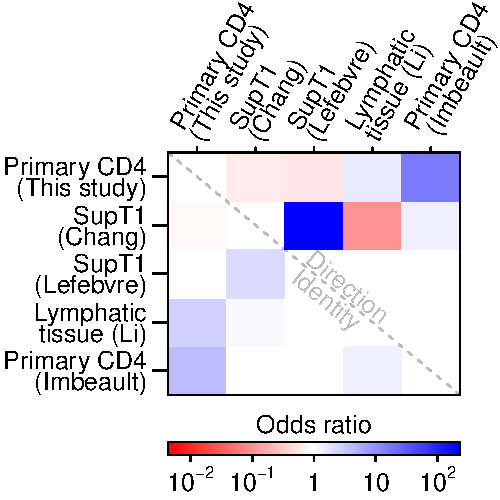
\includegraphics[width=0.5\textwidth]{compare.pdf}
				}{
					\caption[Comparisons among studies quantifying cellular gene expression after HIV infection]{Comparisons among studies quantifying cellular gene expression after HIV infection. For each pair of studies, the association between up- and down-regulation calls was measured for genes identified by both studies as differentially expressed (above the diagonal).  As another comparison, we also measured the agreement between studies for which genes were called differentially expressed regardless of direction (below the diagonal). The color scale shows the conservative (i.e.\  closest to 1) boundary of the confidence interval of the odds ratio with blue indicating a positive association and red a negative association between studies. For confidence intervals overlapping 1, the value was set to 1. Therefore all colored squares indicate significant associations.}	\label{figGenes}
				}
		\end{figure}

	\subsection{Comparison of the HIV infected cell transcriptional profiles to addit\-ional experimental T cell profiles}
		To investigate the transcriptional changes in more depth, we compared the results of the five studies of HIV infection to transcriptional profiles comparing immune cell subsets available at the Molecular Signatures Database (MSigDB) \citep{Subramanian2005}. The MSigDB reports genes that are increased or decreased in relative expression for each of 185 pairs of transcriptional profiles involving \cdFour{} T cells.  We compared the lists of affected genes in each pair to genes altered in activity by HIV infection. Those pairs of studies with the most significant associations with \hivEight{} data are show in Figure \ref{figMsig}A.  For comparison, the associations with the four other HIV transcriptional profiling studies mentioned above are shown as well.

		The most significant associations for our data showed gene expression in \hivEight{}-infected cells moving away from typical T cell expression patterns and towards patterns more similar to B cells, myeloid cells and bulk peripheral blood mononuclear cells (all Fisher's $p<10^{-15}$) (Figure \ref{figMsig}A). These changes were also seen, although to a lesser extent, in the \citet{Imbeault2009} study which also used primary \cdFour{} T cells.

		For comparison, we also extracted those profiles most strongly associated with the transcriptional data on lymphatic tissue of HIV patients \citep{Li2009}. The profiles showed patterns similar to strongly stimulated T cells, autoimmune disease and to the Th1 T cell subset (all $p<0.01$) (Figure \ref{figMsig}B). Our data in primary \cdFour{} T cells paralleled the changes seen in lymphatic tissue. These transcriptional changes again highlights the strong immune response generated by HIV infection in primary cells.
		
		\begin{figure}
			\centering
			\floatbox[{\capbeside\thisfloatsetup{capbesideposition={right,top}}}]{figure}[\FBwidth]{
				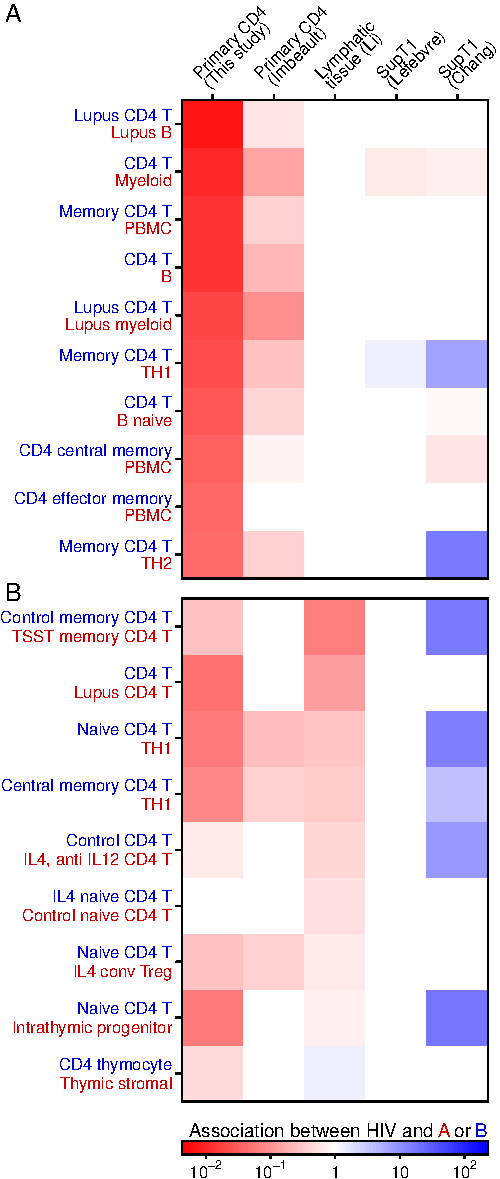
\includegraphics[width=0.5\textwidth]{compareMsig.pdf}
			}{
				\caption[Comparisons of the effect of HIV infection on gene expression to studies comparing subsets of immune cells]{Comparisons of the effect of HIV infection on gene expression to studies comparing subsets of immune cells. The MSigDB database was used to extract 185 sets of differentially expressed genes from pairs of transcriptional profiling studies of immune cell subsets involving \cdFour{} T cells. For each pair of studies, we used Fisher's exact test to measure the association between up- and down-regulation calls for genes identified as differentially expressed in both our HIV study and the comparator immune subsets. A) The transcriptional profiles with strongest associations with changes observed in our study of \hivEight{} infection of primary T cells. Blue indicates an positive association between changes seen in HIV infected cells and the first immune subset (text colored blue) while red indicates a positive association with the second immune subset (text colored red). The color scale shows the conservative (i.e.\  closest to 1) boundary of the confidence interval of the odds ratio. For confidence intervals overlapping 1, the value was set to 1. Therefore all colored squares indicate significant associations. B) As in A, but showing the transcriptional profiles most strongly associated with changes observed in lymph node biopsies from acutely infected patients \citep{Li2009}. }
				\label{figMsig}
			}
		\end{figure}

	
	\subsection{Intron retention} %%%%%%%%%%%%%%%%%%%%%%%%%%%%%%%%%%%%%%%%%%%%%%%%%%%%%%%%%%%%%%%%%%%%%
		Cells respond to infection by shutting down macromolecular synthesis at multiple levels \citep{Iwase1997,Johnstone1998,Williams1999,Ramana2000,Liang2006}, so we investigated whether cells also showed perturbations in splicing efficiency after infection. As a probe, we created a database of cellular genomic regions annotated exclusively as exons or introns in all spliceforms in the UCSC gene database \citep{Hsu2006} and quantified expression in these regions in infected and uninfected cells. We found a significant increase in intronic sequences relative to exonic sequence (Wilcoxon $p<10^{-15}$) (Figure \ref{figIntron}A).  This increase in intronic sequence was reproducible between replicates in our study (Kendall's $\tau$=0.42, $p<10^{-15}$) (Figure \ref{figIntron}B). We reanalyzed RNA-Seq data from \citet{Chang2011} and also documented intron retention which correlated with the changes seen in our data (Kendall's $\tau$=0.12, $p<10^{-15}$) (Figure \ref{figIntron}C).

		A possible artifactual explanation for enrichment of intronic sequences could involve greater DNA contamination in the infected cells samples. That is, if the relative amount of DNA differed between treatments, the amount of apparent intronic sequences could also differ due to sequencing of contaminating DNA. To examine wheth\-er DNA contamination was abundant in our samples, we compiled a collection of 27 large gene desert regions, defined here as 1) regions outside the centrosome and first and last cytoband, 2) containing less than 1\% unknown sequence, 3) containing no genes annotated in UCSC genes \citep{Hsu2006}, 4) containing no repeats annotated in the repeatMasker database \citep{Jurka2005} and 5) spanning more than 100 kb. No reads were mapped to these 41 Mb of gene deserts in any sample, arguing against explanations based on DNA contamination. Thus these data indicate that intron retention was increased in these cell populations upon HIV infection, revealing a previously undisclosed aspect of the host cell transcriptional response to infection.
		
		  Previous studies have reported changes in the expression and localization of splicing factors with HIV infection \citep{Maldarelli1998,Dowling2008,Monette2009}. In our data, \hivEight{} infection significantly altered the expression of genes involved in RNA splicing ($p=2\times10^{-7}$) and nonsense-mediated decay ($p<10^{-15}$). Genes related to nonsense-mediated decay genes showed a strong pattern of lowered RNA abundance, with 71 out of 118 annotated genes significantly lower in expression after infection. These patterns suggest potential mechanisms for the intron retention observed here.
		
		\begin{figure}
			\centering
				\includegraphics[width=\textwidth]{intronCombo.pdf}
			\caption[Changes in the abundance of intronic regions with HIV infection]{Changes in the abundance of intronic regions with HIV infection. Expression of intronic and exonic regions was quantified as the proportion of reads mapping within the intron/exon out of the total reads mapping to the transcription units overlapping that intron/exon. A) Comparison of the ratios of expression between infected and uninfected replicates in exclusively intronic or exonic regions of transcription units. B) Reproducibility of intron retention between replicates. Each point quantifies the change in expression with HIV infection for a specific intronic region. The x-axis shows shows changes in gene activity accompanying infection for one set of replicates (Infected-1 and Infected-2 vs. Uninfected-1) and the y-axis shows the same data for different replicates (Infected-3 vs. Uninfected-2). C) Reproducibility of intron retention between studies. The plot is arranged as in B but with all data from our study combined on the x-axis and corresponding data from \citet{Chang2011} on the y-axis.}
			%Retention of introns and activation of repeated sequence associated with HIV89.6 infection of primary T cells. A) The ratios of expression between infected and uninfected replicates in exclusively intronic or exonic regions of transcription units.  Comparison of representation of introns and exons in the infected and uninfected samples.  B) An example of intron retention in the cellular gene. } 
			\label{figIntron}
		\end{figure}

	\subsection{Induction of transcription from HERVs and LINEs by \hivEight{} infection}
		HIV infection has been reported to induce expression of certain HERVs, particularly HERV-K \citep{Contreras-Galindo2007,Contreras-Galindo2013,Bhardwaj2014}, and LINE and Alu transposable elements \citep{Jones2013}, providing candidate markers of infection and possible vaccine targets.  Thus we analyzed our data in primary T cells infected with \hivEight{} to investigate the expression of HERVs, LINEs and other repeated sequences.  Figure \ref{figHervs}A shows a comparison of the association between changes in expression with \hivEight{} infection and the various genomic repeat types over varying levels of differential expression. At high levels of expression, ERV-9  (odds ratio at $4\times$ expression: 152, 95\% CI:82.5--259) and its long terminal repeat LTR12C  (odds ratio at $4\times$ expression: 144, 95\% CI: 98.2--207) are the only repeats highly associated with upregulation during HIV infection. Looking at genomic repeats with any significant increase, the expression of many recently acquired genomic repeats, including L1HS, LTR5\_Hs (a human specific LTR of HERV-K), AluYa5, AluYg6 and SVA\_D and SVA\_F, were associated with \hivEight{} infection (Figure \ref{figHervs}B). 
		
		We saw a relationship between the age of genomic repeats and its likelihood of being induced by \hivEight{} infection. The most highly enriched repeats were associated with relatively recent hominid-specific repeat classes as annotated by the RepeatMasker database (repeat classes with $p<10^{-50}$ odds ratio: 31.6, 95\% CI: 8.88--112). In HERV-K (HML-2), the most recently active endogenous retrovirus in the human genome \citep{Medstrand1998,Macfarlane2004,Subramanian2011}, we saw that integrations unique to the human genome \citep{Subramanian2011} were more likely to be differentially expressed than older HERV-Ks (odds ratio: 5.38, 95\% CI: 1.93--16.0). 

		Previous RNA-Seq studies of cellular expression during HIV infection in transformed cell lines did not report increases in HERV mRNA \citep{Lefebvre2011,Chang2011}. To investigate this difference, we downloaded and analyzed the RNA-Seq data from \citet{Chang2011}, which quantified gene activity in transformed SupT1 cells infected with a lab-adapted strain of HIV.  We found a much higher level of HERV expression in their data in both HIV infected cells and uninfected controls than in primary cells (Figure \ref{figHervs}C). We suspect that in SupT1 cells, as with many cancerous cells \citep{Buescher2005,Howard2008,Iskow2010,Lee2012,Criscione2014}, the baseline expression of transposons and endogenous retroviruses is higher than in primary cells, masking further induction by HIV infection.

		\begin{figure}
			\centering
				\floatbox[{\capbeside\thisfloatsetup{capbesideposition={right,top}}}]{figure}[\FBwidth]{
					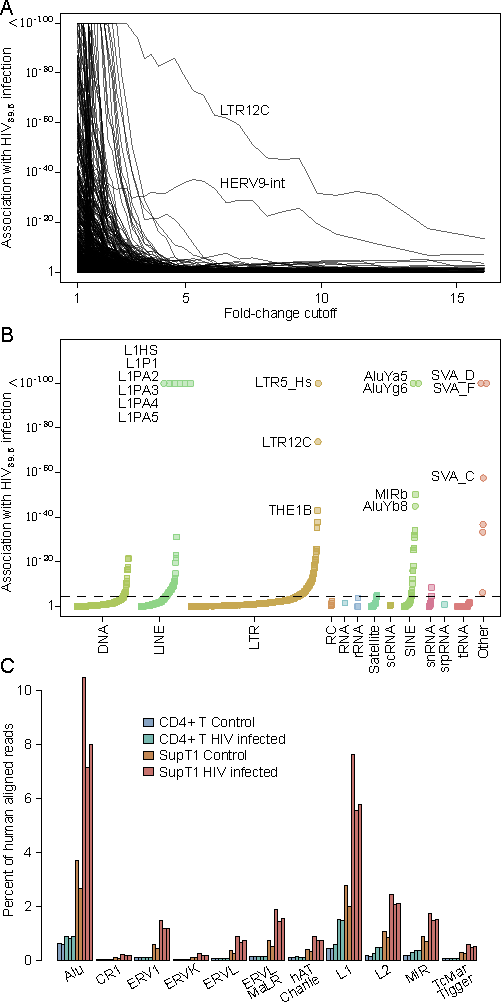
\includegraphics[width=0.5\textwidth]{ltrCombo.pdf}
				}{
					\caption[Repeat categories enriched upon infection with HIV]{Repeat categories enriched upon infection with HIV. A) The association of repeat regions differentially expressed after \hivEight{} infection of primary T cells observed for varying thresholds of differential expression. The threshold used to call a gene differentially expressed based on the Bayesian posterior median was varied and Fisher's exact test was used to assess whether any genomic repeats had a significant association with this differential expression. Note that only ERV-9 (annotated as HERV9-int in the RepeatMasker database) and it's corresponding long terminal repeat LTR12C were significantly associated with large changes in expression. B) Enrichment of repeat categories in regions differentially expressed (Bayesian 95\% credible interval \textgreater{}1) between HIV-infected and control \cdFour{} T cells. The repeated sequences are ordered on the x-axis by the extent of induction within each class, the y-axis shows the p-value for upregulation after infection. The dashed line indicates a Bonferroni corrected $p$ value of 0.05. (C) The proportion of human mapped reads that align within classes of genomic repeats for data from primary \cdFour{} T cells from this study and SupT1 cells from \citet{Chang2011}. A single read mapping multiple times to a given category was only counted once.}
					\label{figHervs}
				}
		\end{figure}

		We observed heterogeneous expression among ERV-9/LTR12C sequences and so investigated the primary sequence determinants. We observed that ERV-9/LTR12C has three variants of differing length in the U3 region just upstream of the transcription start site (Figure \ref{figLtr12c}A), an important region for transcription initiation \citep{LaMantia1992}.  The U3 region of LTR12C also contains multiple motifs for transcription factors NFY, GATA2 and MZF1 \citep{Yu2005}. To clarify factors affecting expression levels, we counted the number of motifs matching these transcription factors, assigned each LTR12C to one of the length classes, counted the number of mutations away from the consensus for that length class and checked for integration in a transcription unit. We then carried out a regression analysis to test the effects of these variables on LTR12C differential expression. We found that \hivEight{} induced transcription was more likely with the fewer mutations away from consensus, the number of locations matching the NFY transcription factor binding motif (CCAAT) and LTRs containing the short length variant of the \threePrime{} U3 region. The presence of a MZF1 motif near the transcription start site decreased transcription (Figure \ref{figLtr12c}B). 
		
		\begin{figure}
			\centering
				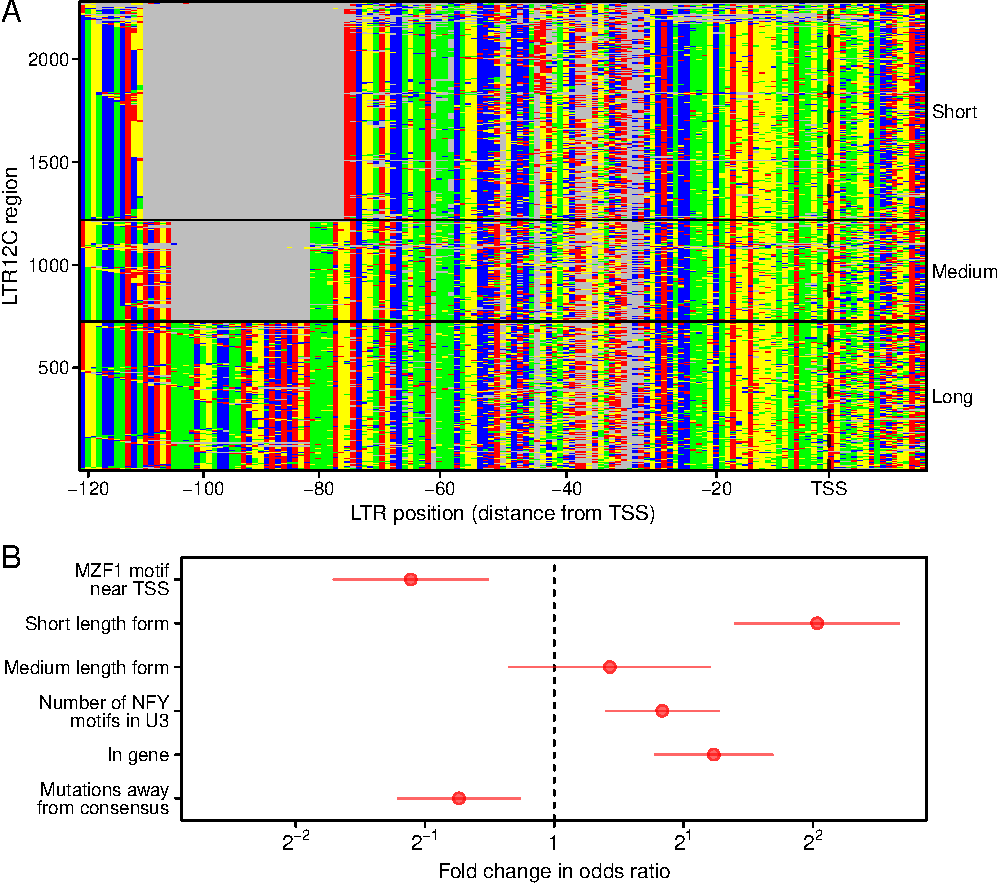
\includegraphics[width=\textwidth]{ltr12c.pdf}
			\caption[Characteristics of LTR12C sequences associated with induction upon infection with \hivEight{}]{Characteristics of LTR12C sequences associated with induction upon infection of primary T cells with \hivEight{}.  A) An alignment of the \threePrime{} end of the U3 region of repeats annotated as ERV-9 LTR12C. Each row is a LTR sequence and each column a base in that sequence colored by nucleotide identity. Three distinct classes are visible with a short, medium and long form. Mutations away from the consensus can also be seen. B)  The coefficients (points) and $\pm$1.96 standard errors (horizontal lines) of a logistic regression comparing differential expression of LTR12C to the presence of MZF1 and NFY motifs, short/medium/long length alternate forms of the U3-R region, mutations away from the consensus for each length form and integration inside a transcription unit. The coefficient shown for mutations away from consensus is for a 10 mutation difference and the coefficient shown for NFY motifs is for a change of 5 additional motifs. All other coefficients are for binary values.}
			\label{figLtr12c}
		\end{figure}

	\subsection{HIV mRNA synthesis and splicing} %%%%%%%%%%%%%%%%%%%%%%%%%%%%%%%%%%%%%%%%%%%%%%%%%%%%%%%%%%%%%%%%%%%%%  
		Over 24 million Illumina reads mapped to \hivEight{}, yielding an average coverage of over 240,000-fold.  Reads mapping to \hivEight{} comprised between 3.4--4.8\% of mapped reads in the infected samples (Table \ref{tabSamples}). Assuming HIV-infected cells contain the same amount of mRNA as uninfected cells and adjusting for rates of infection ranging between 21--37.5\% (Table \ref{tabSamples}), we estimate that HIV transcripts comprise between 13.0--16.2\% of the total polyadenylated mRNA nucleotides in infected cells 48 hours after initial infection. This parallels previous estimates of around 10\% \citep{Whisnant2013} at 48 hours postinfection, 38\% at 24 hours \citep{Chang2011} or 30\% after 72 hours \citep{Corbeil2001}. %could be underestimates due to 3' bias

		Over 47,257 single reads spanned previously reported HIV splice junctions, allowing a quantitative assessment of donor and acceptor utilization (Figure \ref{figHiv}A). As expected from previous studies \citep{Purcell1993,Ocwieja2012}, the most abundant junctions were D1-A5 and D4-A7.  We confirmed the use of unusual splice acceptors A8c and A5a, previously reported in \hivEight{} \citep{Ocwieja2012}. In our data, we also see a higher abundance of D1-A1 and D1-A2 splice junctions than might be expected \citep{Purcell1993,Ocwieja2012}, although previous studies reported proportional abundance within size classes, making comparisons between size classes uncertain. % and observed that A8c is the most commonly used acceptor for the D4 donor that forms the 2 kb and 1 kb size class.

		A \threePrime{} bias is apparent in our sequencing data (Additional file 5). This could be due to the poly-A capture step of the protocol where any break in the RNA would result in distal \fivePrime{} sequences being lost \citep{Lahens2014}. We used sequence reads from the large unspliced HIV intron 1 to measure this bias using a regression of the $\log$ of the number of fragments with a \fivePrime{}-most end starting at a given position against the distance of that position from the viral polyadenylation site, yielding an estimated probability of breakage of 0.021\% per base (Additional file 5). Given this rate of termination, there is only a 14\% chance of reaching the \fivePrime{} end of the 9171 nt unspliced HIV genome (\((1-0.00021)^{9171}\)). 


		\begin{figure}
				\centering
				\floatbox[{\capbeside\thisfloatsetup{capbesideposition={right,top}}}]{figure}[\FBwidth]{
					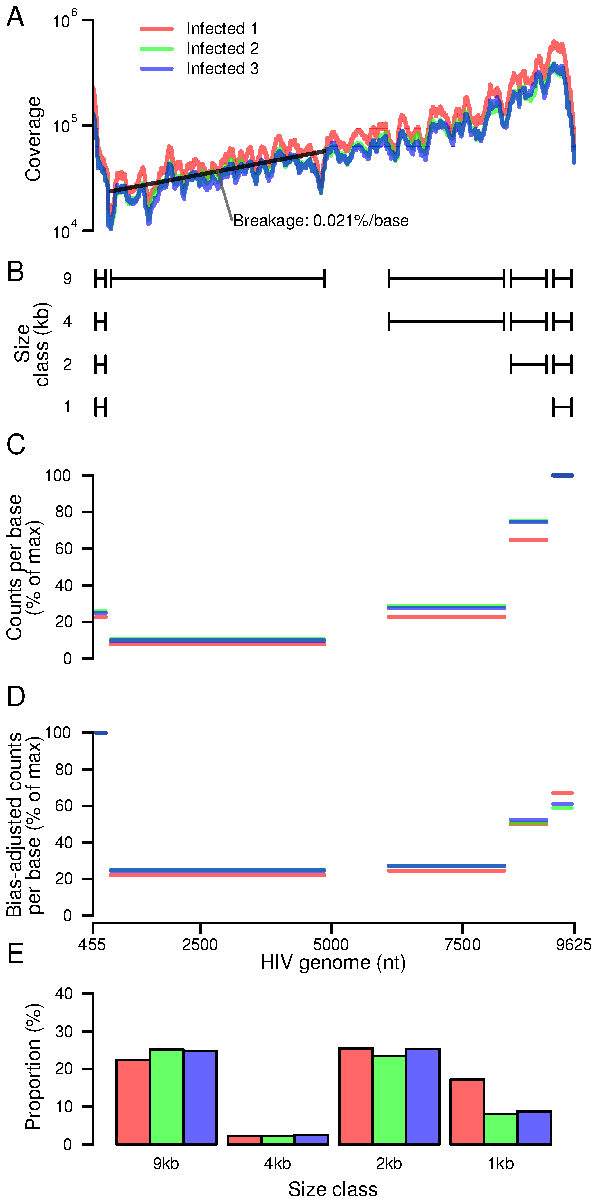
\includegraphics[width=0.6\textwidth]{additionalFile5.pdf}
				}{
					\caption[Estimating relative abundance of \hivEight{} message size classes using RNA-Seq data]{
						Estimating relative abundance of \hivEight{} message size classes using RNA-Seq data.\\
						A) RNA-Seq coverage of the \hivEight{} genome for the replicates in this study. Each replicate is indicated by a different color. The HIV genome is shown on the x-axis and the number of reads that aligned to each position is shown on the y-axis. Black line indicates the 0.021\% coverage decrease per base distance from the \threePrime{} end of the mRNA estimated from a least squares fit on the read counts in the first intron.\\
						B) Diagram of the segments of the \hivEight{} RNA present in each of 9 kb, 4 kb, 2 kb and 1 kb size class. \\
						C) The proportion of reads mapped to each of the segments of the \hivEight{} genome shown in B adjusted by the length of the segment. Each replicate is shown by a different color.\\
						D) Corrected representation of RNA segments from the different size classes. Because cDNA synthesis was primed from the polyA tail, more \threePrime{} sequences are recovered preferentially. Using the bias estimate from A, we adjusted each genome segment by the inverse of the bias predicted based on its distance from the \threePrime{} end of the mRNA. Corrected proportions for the indicated RNA segments are shown colored by replicate. \\
						E) The proportion of each size class was inferred using the estimates in D by calculating the difference between segments. Replicates are indicated by color.
				}
					\label{figCalculations}
				}
		\end{figure}

		\citet{Ocwieja2012} determined the relative abundance of \hivEight{} of similarly sized transcripts using PacBio single molecule sequencing, but were not able to estimate the relative abundance of all transcripts due to a sequencing bias favoring shorter transcripts.  For this reason, relative abundances could only be specified within message size classes (i.e.\  the 4 kb, 2 kb and unexpectedly a 1 kb size class as well) and the overall quantitative abundances were unknown.  The RNA-Seq data reported here are unable to determine complete transcript abundance because the short read length does not allow reconstruction of multiply spliced messages but do permit estimation of size class abundances after correcting for \threePrime{} bias (Additional file 5). Thus the PacBio data reported by \citet{Ocwieja2012} and the Illumina data reported here can be combined together to determine complete relative abundance of all \hivEight{} transcripts (Figure \ref{figHiv}B). 

	   The most abundant HIV mRNAs were the unspliced HIV genome (37.6\%), a transcript encoding Nef (D1-A5-D4-A7: 15.5\%), two 1 kb size class transcripts (D1-A5-D4-A8c: 10.6\%, D1-A8c: 4.9\%) and two Rev-encoding transcripts (D1-A4c-D4-A7: 4.2\%,D1-A4b-D4-A7: 3.1\%). The function of this large amount of 1 kb transcript is unknown. These two 1 kb transcripts do not appear to encode significant open reading frames although other 1 kb transcripts can encode a Rev-Nef fusion \citep{Ocwieja2012}. 

		Using these abundances, we can estimate the number of \hivEight{} genomes in these pri\-mary T cells 48 hours after infection.  To determine the proportion of the mRNA nucleotides from viral transcripts, we multiplied the estimated abundances by their tran\-script lengths. Unspliced genome tran\-scripts appear to form 79\% of the mRNA nucleotides from \hivEight{} transcripts. Assuming T cells contain at least 0.1 pg of mRNA then an infected cell should contain at least 0.011 pg of unspliced HIV transcript ($0.1 \textrm{pg} \times 0.14\frac{\textrm{HIV mRNA nt}}{\textrm{cell mRNA nt}}\times 0.79\frac{\textrm{unspliced mRNA nt}}{\textrm{HIV mRNA nt}}$) or, assuming 9171 bases of RNA weigh about $5 \times 10^{-6}$ pg, at least 2200 HIV genomes at 48 hour post infection. This estimate rough\-ly agrees with previous estimates of HIV production per cell \citep{Hockett1999,DeBoer2010,Whisnant2013}. 

		\begin{figure}
			\centering
				\floatbox[{\capbeside\thisfloatsetup{capbesideposition={right,top}}}]{figure}[\FBwidth]{
					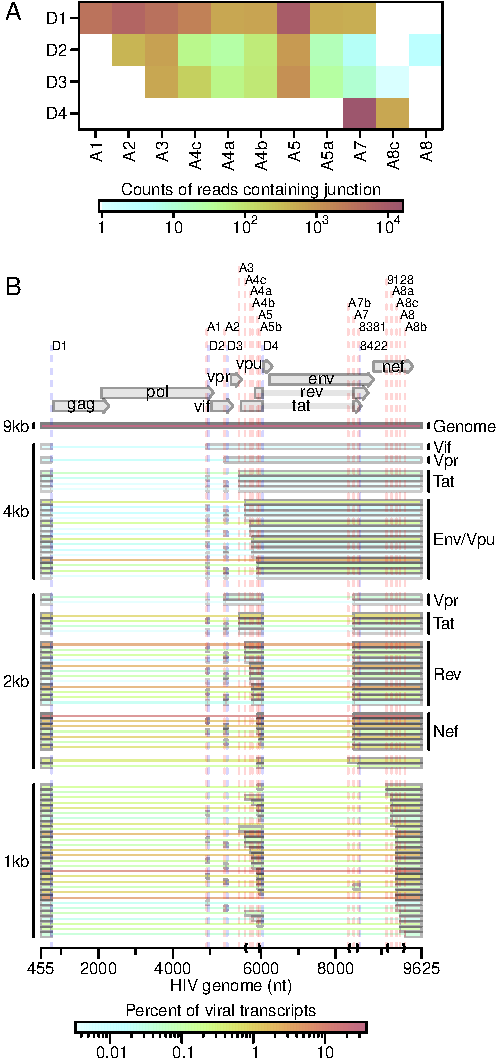
\includegraphics[width=0.5\textwidth]{comboHiv.pdf}
				}{
					\caption[Transcription and splicing of the \hivEight{} RNA]{Transcription and splicing of the \hivEight{} RNA. A) Junctions between HIV splice donors and acceptors observed in the RNA-Seq data. Acceptors are shown as the columns and donors as the rows with the coloring indicating the frequency of each pairing.   B) The relative abundance of all \hivEight{} transcripts as determined by a combination of PacBio sequencing \citep{Ocwieja2012} and Illumina sequencing. Message structures were generated by targeted long read single molecule sequencing, which allowed association of multiple splice junctions in single sequence reads. The Illumina short read sequencing allowed normalization of message abundances between size classes. The inferred HIV message population is shown colored by relative abundance.} 
					\label{figHiv}
				}
		\end{figure}

	\subsection{Human-HIV chimeric reads} %%%%%%%%%%%%%%%%%%%%%%%%%%%%%%%%%%%%%%%%%%%%%%%%%%%%%%%%%%%%%%%%%%%%%
		The suggestion that HIV integration may disrupt cellular cancer-associated genes and thereby promote cell proliferation \citep{Ikeda2007,Wagner2014,Maldarelli2014,Cohn2015} has focused attention on the range of novel message types formed when HIV integrates within transcription units \citep{Schroder2002,Wang2007,Brady2009,Sherrill-Mix2013,Marini2015}. Chimeric reads containing HIV and cellular sequence are also of clinical interest due to the potential of lentiviral vectors to trigger oncogenesis in gene therapy patients through insertional mutagenesis \citep{Cavazzana-Calvo2010,Hacein-Bey-Abina2008,Moiani2012,Cesana2012}. 
		
		In our data, 80,045 reads contained sequences matching to both HIV and human genomic DNA, but a considerable complication arises because chimeras can be formed artifactually during the preparation of libraries for sequence analysis \citep{Paeaebo1990,Odelberg1995,Zeng2002,Tasic2002,Geiszt2004,Cocquet2006,McManus2010,Cogne2014}. Many of the chimeric sequences in our data contained junctions between the HIV and human sequence where the ends of the human and HIV sequence were similar and potentially complementary (Figure \ref{figChimera}A). This raises the concern that some of these chimeras could be products of in vitro recombinations during the reverse transcription, amplification and sequencing processes. Template switching between sequences with shared similarity is a well established property of retroviral reverse transcriptase enzymes used in RNA-Seq library preparation \citep{Gilboa1979,Luo1990,Houseley2010}. Priming off incomplete transcripts during DNA synthesis is another potential source of chimeric transcripts \citep{Paeaebo1990,Meyerhans1990,Odelberg1995,Lahr2009}. Failing to account for chimeras can hinder interpretation of deep sequencing data \citep{Zeng2002,Tasic2002,Geiszt2004,Cocquet2006,McManus2010,Cogne2014}.

		Also consistent with artifactual chimera formation, 7,354 reads (9.2\%  of chimeric messages) contained HIV sequences joined to human mitochondrial sequences, yet HIV proviruses have not previously been found integrated in mitochondrial DNA \citep{Wang2007}. To probe this further, we used ligation-mediated PCR to recover integration site junctions from the same infected cell populations analyzed by RNA seq, yielding \nIntegrations{} unique integration sites (Figure \ref{figChimera}B) \citep{Berry2014}.  No integrations in mitochondrial DNA were detected. We conclude that chimeric HIV-mitochondrial sequence reads in the RNA-seq data represent artifacts of library construction and so used these chimeras as an assay to evaluate subsequent data filtering steps.  We reasoned that reads without sequence similarity at junctions between human and HIV mapping were less likely to be artifacts caused by template switching. Filtering to only reads where no overlap and no unknown intervening sequence was present between human and HIV portions left 2181 junctions and reduced the proportion of reads containing mitochondrial DNA to 2.4\%. Of the remaining HIV-human chimeric reads, the HIV portion of 605 sequences bordered the \threePrime{} or \fivePrime{} end of HIV or an HIV splice donor or acceptor. Filtering to these more likely authentic junctions left only 2 (0.3\%) chimeric reads containing mitochondrial sequence. This decrease in likely mitochondrial artifacts suggests that the filtering was effective. The high rate of mitochondrial chimeras in the unfiltered sequences raises the concern that artifacts may easily distort results in studies using similar amplification and sequencing techniques.

		Chimeric messages composed of HIV and cellular RNA sequences can be formed by cellular gene transcription reading into the integrated provirus, by HIV transcription reading out through the viral polyadenylation site or by splicing between human and viral splice sites. In our filtered data, the predominant forms appear to be derived from reading through the HIV polyadenylation signal into the surrounding DNA (78\%), splicing out of the viral D4 splice donor to join to human slice acceptors (17\%) and reading into the HIV \fivePrime{} LTR from human sequence (4.0\%) (Figure \ref{figChimera}C). No splice site other than D4 had more than two chimeric reads observed. 
		
		The filtered chimeric reads had many traits consistent with biological chimera formation. The reads containing HIV D4 joined to human sequences had the characteristics expected of splicing---72.1\% of the chimeric junctions mapped to known human acceptors and 96.1\% mapped to a location immediately preceded by the AG consensus of human mRNA acceptors. The reads containing the \fivePrime{} or \threePrime{} LTR border were almost exclusively (93\%) found in transcription units, with odds of being in a gene 2.3-fold (95\% CI: 1.6--3.2$\times$) higher than integration sites from the same sample. The \fivePrime{} or \threePrime{} chimeras were also more likely to be located in an exon than integration sites even after excluding any integration or chimera not located in a transcription unit (odds ratio: 2.1$\times$, 95\% CI: 1.6--2.6$\times$).
		%Reads containing a junction of the HIV \threePrime{} end with human sequence appear to be more common than reads containing a junction of the HIV \fivePrime{} end but this conclusion is tentative due to \threePrime{} sequencing bias and uncertainty of strand of origin.

		%these chimeric sequence would be originating from and where they would be polyadenylated. In addition, since HIV transcripts form a large proportion of mRNA transcriptions and at most a handful of genes in each infected cell could be situated appropriately to even be able to read into an integrated provirus, these differences in abundance might be biased by the opportunity for polymerase to even encounter the sequences involved. Proviral expression would likely be lower in vivo in cells that don't quickly succumb to infection or in cells transduced by lentiviral vectors. 

		 We next compared whether the human and viral segments of chimeric reads agreed or disagreed in orientation (i.e.\  strand transcribed) for reads with the human portion mapped within annotated transcription units. The sequencing technique used here does not preserve strand information, but we can check whether the strand of a sequence read agrees or disagrees with the annotated gene strand and compare this to the observed strand of the HIV portion of the read. We found a strong association between the orientation of the human and HIV portions of chimeric reads within \threePrime{} and \fivePrime{} chimeras (odds ratio: 6.2$\times$, 95\% CI: 3.9--10.2$\times$). This highly significant enrichment of HIV and human genes in the same orientation (Fisher's exact test $p<10^{-15}$) might indicate that antisense HIV RNA is rapidly degraded by a response to double-stranded RNA or that polymerases oriented in opposing directions interfere with one another during elongation. Chimeras involving HIV splice donor D4 were even more highly enriched for matching orientations (odds ratio: 52.5$\times$, 95\% CI: 12.1--307$\times$) suggesting that pairing with human splice acceptors may add an additional constraint on the orientation of D4 chimeric reads.

		 %We found a strong association between the orientation of the HIV and human portions of chimeric reads with the odds of the agreement between the two portions 6.3-times higher (95\% CI: 3.9--$10.2\times$) than the odds of being in opposite orientations. 

		Based on these data, we can propose a lower bound on the relative abundance of chimeras. If we assume that our filtering removed nearly all artifacts so that we have few false positives, then our estimate should be lower than the true proportion of chimeras. In our data, only $\frac{604}{\nHIVFrag{}} = 0.0048\%$ of reads containing sequence mapping to HIV also contained identifiable chimeric junctions. However, this is an underestimate because in an HIV-derived mRNA, any fragment of the sequence will be mappable to HIV, while for a chimeric sequence only a read spanning the HIV-human junction will allow identification of a chimera. If we assume that 25 bases of sequence are necessary to map to human or HIV sequence, then, with the 100-bp reads used here, only read fragments starting between 75- and 25-bp downstream of the chimeric junction will be identifiable. If we assume the average chimeric mRNA sequences is at least 2 kb long, then a read from a chimeric sequence has at most a $\frac{50}{2000}=2.5\%$ chance of containing a mappable junction. Thus, a lower bound for the proportion of HIV mRNA that also contain human-derived sequences is 0.2\% ($\frac{0.0048\textrm{\%}}{2.5\%}$). Looking only at splicing from HIV donor D4, we saw 16,843 reads containing a junction from D4 to an HIV acceptor and 104 reads from D4 to human sequence. Thus, in our data, 0.6\% of D4 splice products form junctions with human acceptors instead of HIV acceptors.


		\begin{figure}
				\centering
				\floatbox[{\capbeside\thisfloatsetup{capbesideposition={right,top}}}]{figure}[\FBwidth]{
					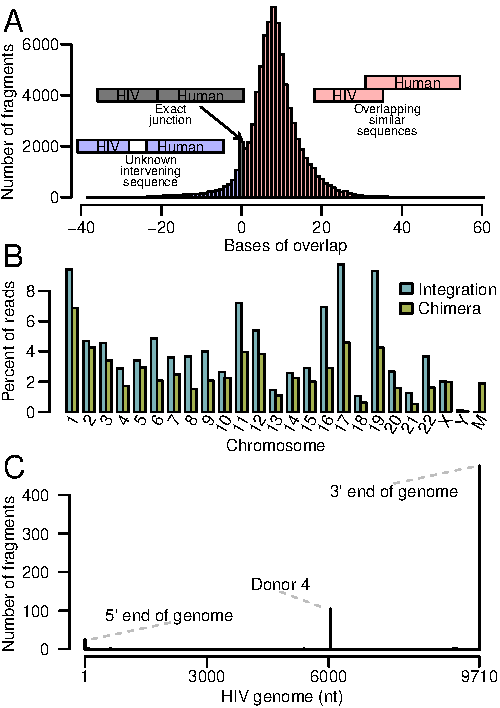
\includegraphics[width=0.5\textwidth]{chimeraCombo.pdf}
				}{
					\caption[Chimeric RNA sequences containing both human and HIV sequences]{Analysis of chimeric RNA sequences containing both human and HIV sequences. A) The length of overlapping sequence (regions of complementarity potentially favoring chimera formation) matching both human and HIV at inferred chimeric junctions. The x-axis shows the length of the overlap and the y-axis shows the frequency of chimeric junctions with the indicated extent of overlap.  B) Chromosomal distribution of uniquely mapping HIV integration sites from the same infections of primary T cells and comparison to uniquely mapping human sequences in chimeric reads observed in RNA-Seq. Note that the mitochondrial genome, denoted as M, has no authentic integration sites but does have extensive matches to chimeric junctions found in the RNA-Seq data. C) Counts of the location in the HIV genome of the HIV-human junctions in filtered chimeric reads.} % CHECK ONLY BEST HIV MATCH]]
					\label{figChimera}
				}
		\end{figure}



\section{Discussion}
	Here we used RNA-Seq to analyze mRNA accumulation and splicing in primary T cells infected with the low passage isolate \hivEight{}.  We did not carry out dense time series analysis, compare different human cell donors or compare different perturbations of the infections---instead, we focused on generating a dense data set at a single time point.  We analyzed replicate infected cell and control samples to allow discrimination of within-condition versus between-condition variation and assessed differences using a series of bioinformatic approaches. Many previous studies have used microarray technology or RNA-Seq to study gene activity in HIV-infected cells \citep{Corbeil2001,delaFuente2002,Mitchell2003,Woelk2004,Hyrcza2007,Wu2008,Smith2010,Chang2011,Lefebvre2011,Imbeault2012,Mohammadi2013,Peng2014}, usually analyzing infections of transformed cell lines or laboratory adapted strains of HIV-1. Here we present what is to our knowledge the deepest RNA-Seq data set reported for infection in primary T cells using a low passage HIV isolate (\hivEight{}). This data set was paired with a set of \nIntegrations{} unique integration site sequences extracted from the same infections, which were critical to our ability to quality control chimeric reads. An advantage of studies using cell lines and laboratory adapted strains is that often a high percent of cell infection can be achieved, whereas in this study we achieved only $\approximately$30\% infection.  However, we report distinctive features of the transcriptional response not seen in studies of HIV infections in cell lines.  Novel in this study are 1) identification of intron retention as a consequence of HIV infection, 2) the finding of activation of ERV-9/LTR12C after HIV infection,  3) generation of a quantitative account of the structures and abundances of over 70 \hivEight{} messages and 4) clarification of the predominant types of HIV-host transcriptional chimeras.  These findings are discussed below.

	Broad changes in host cell mRNA abundances were evident after infection, with over 17\% of expressed genes changing significantly in activity. Changes included expected response to viral infection, apoptosis and T cell activation. Although it is not possible here to separate the response of infected and bystander cells, this study highlights the drastic changes in cellular expression caused by HIV-1 infection. In a meta-analysis including four previously published studies, no gene was detected as differentially expressed in all five studies and only a handful of genes appeared in four out of five studies. Further analysis showed that expression changes appear to be cell type specific, raising concerns that studies using cell lines may not fully reflect host cell responses in \emph{in vivo} infections. 

	Unexpectedly, intronic sequences were more common in the RNA-Seq data from cells after \hivEight{} infection than in mock infected cells.  The mechanism is unclear.  It is possible that the splicing machinery is reduced in activity after 48 hours of infection, perhaps as a part of the antiviral response of infected and bystander cells.  HIV infection does appear to alter expression and localization of some splicing factors \citep{Dowling2008,Monette2009}. In addition, we saw a large reduction in the abundance of mRNA from nonsense-mediated decay related genes, perhaps indicating that RNA surveillance is loosened thus allowing more unspliced or aberrantly spliced transcripts.  Alternatively, fully spliced mRNAs might be more rapidly degraded after infection, possibly by interferon-mediated induction of RNaseL \citep{Al-Ahmadi2009}.  A speculative possibility is that \hivEight{} encodes a factor that alters cellular splicing or promotes mRNA degradation to optimize splicing and translation of viral messages.

	Infection resulted in increased expression of specific cellular repeated se\-quences. HERVs, in particular HERV-K, have previously been observed to show increased RNA accumulation with HIV infection \citep{Contreras-Galindo2007,Jones2012,Contreras-Galindo2013,Bhardwaj2014} and possibly represent vaccine targets because of their production of distinctive proteins \citep{Boller1997,Buescher2005,Garrison2007,Tandon2011,SenGupta2011,Jones2012}.  Here, though we saw modest increases in HERV-K expression, ERV-9 had the greatest change in expression (33 LTR12C and 14 ERV-9 annotated regions with greater than $4\times$ change in expression). Previous RNA-Seq studies of HIV infection in cell lines did not report increases in HERV expression \citep{Chang2011,Lefebvre2011} but this difference is likely due to a much higher baseline expression of HERVs in transformed cell lines. We also observed increases in LINE and Alu element transcription, as has been reported previously \citep{Jones2013}, and expression changes in ERV-9/LTR12C expression associated with transcription factor motifs and U3 variants.

	Many of the repeated sequence elements that were induced by \hivEight{} infection are relatively recently integrated in the human genome.  The reason for this pattern is unclear.  It may be that older elements have accumulated more mutations, resulting in an inactivation of transcriptional signals.  Alternatively, perhaps the elements that are induced have been recruited for transcriptional control of cellular functions, so that their transcriptional activity is preserved evolutionarily  \citep{Ling2002,Pi2004,Zhang2006}.

	Comparison of results of sequencing \hivEight{} messages using long-read single molecule sequencing (Pacific Biosciences) and dense short read sequencing (Illumina data reported here) allowed a full quantitative accounting of more than 70 \hivEight{} splice forms.  The full length unspliced HIV RNA comprised 37.6\% of all messages, corresponding to about 2000 genomes per cell. Notably abundant messages included those encoding Nef (D1-A5-D4-A7: 15.5\%) and two Rev-encoding transcripts (D1-A4c-D4-A7: 4.2\%,D1-A4b-D4-A7: 3.1\%).  The full set of messages is summarized in Figure \ref{figHiv}B. Our previous analysis revealed an unusually prominent 1 kb size class. \hivEight{} encodes a rare splice acceptor (A8c) within Nef responsible for formation of the short messages.  Our data indicated that two members of the 1-kb size class, D1-A5-D4-A8c and D1-A8c, accounted for 10.6\% and 4.9\% of all messages. The  1 kb size class as a whole accounted for fully 20\% of messages. Most HIV/SIV variants appear to encode an acceptor near this position, suggesting a potential unknown function for these short spliced forms \citep{Smith1992,Carrera2010,Ocwieja2012}.

	After filtering, we detected a sizeable number of apparently authentic chimeras containing both HIV and cellular sequences, allowing comparison to examples of host-cell modification by integration. Mechanisms of insertional activation have been studied intensively in animal models of transformation and in adverse events in human gene therapy. One of the most common mechanisms involves insertion of a retroviral enhancer near a cellular promoter, so that the rate of initiation is increased and normal cellular messages are increased in abundance. However, another common mechanism involves formation of chimeric messages involving both cellular and viral/vector sequences. In HIV infection, examples of insertion in the Bach2 and MKL2 genes have been associated with long term persistence of particular cell clones \citep{Ikeda2007,Maldarelli2014,Wagner2014,Cohn2015}. In these cells, proviruses were integrated within the cellular transcription unit, and the transcriptional direction of the integrated provirus was the same as that of Bach2 or MKL2. This would allow formation of a fusion of the \fivePrime{} HIV sequences with \threePrime{} Bach2 sequences, potentially involving the most common events seen here (either \threePrime{} read out or splicing from HIV D4 to a cellular exon). However, a closely studied example of clonal expansion in a successful lentiviral vector gene therapy for beta-thalassemia was associated with expansion of a cell clone harboring an integrated vector within the transcription unit of HMGA2. In this case the message spliced into the vector and terminated, removing a negative regulatory sequence normally present in the \threePrime{} end HMGA2 message \citep{Cavazzana-Calvo2010}. A targeted study in vitro of chimeric message formation by lentiviral vectors showed examples of multiple types of read-in and -out and splice-in and -out \citep{Moiani2012}, which may have been more frequent and more varied than for \hivEight{} proviruses studied here. The lack of splicing or reading into HIV in this study may be a reflection of the high rate HIV transcription in these infected cells--because HIV was so highly expressed, there would be more opportunities for polymerase to splice out of or read through the HIV genome than to read or splice in. The vast majority of HIV proviruses in expanded clones in well-suppressed patients now appear to be defective \citep{Cohn2015}---going forward, it will be of interest to investigate whether these HIV proviruses are damaged in ways that promote formation of chimeric transcripts. 

	Lastly, we note that several features of the transcriptional response to \hivEight{} infection were suggestive of de-differentiation away from T cell specific expression patterns. The increase in expression of cellular HERVs and LINEs is characteristic of cells in early development. Specific HERVs and transposons, including ERV-9/LTR12C and HERV-K, have been implicated in regulating gene activity early in development \citep{Ling2002,Pi2004,Santoni2012,Fuchs2013,Fort2014,Wang2014}. Several genes related to other hematopoietic cell types showed elevated RNA abundance after \hivEight{} infection. These data are of interest given the finding that patients undergoing long term ART can contain long lived T cell clones that may contribute to the latent reservoir \citep{Joos2008,Brennan2009,Wagner2013,Kearney2014,Cohn2015}.  Possibly the transcriptional responses seen in infected primary T cells here are reflective of processes leading to formation of the long-lived latently-infected cells with stem-like properties.

\section{Conclusions}
	Infections of primary T cells with a low passage HIV isolate show several distinctive features compared with previously published data using T cell lines and/or lab-adapted HIV strains. We found strong changes in expression in genes related to immune response and apoptosis similar to studies of HIV infection in patient samples and primary cells but different from studies performed in SupT1 cell lines. Notable changes after infection included intron retention and activation of recently integrated retrotransposons and endogenous retroviruses, in particular LTR12C/ERV-9. We also present complete absolute estimation of over 70 messages from \hivEight{} and specify the major virus-host chimeras as read out from the \threePrime{} end of the provirus and splicing from viral splice donor 4 to cellular acceptors.


\section{Availability of supporting data}
	RNA-Seq reads from this study are available at the Sequence Read Archive under accession number SRP055981. The integration site data is available at the Sequence Read Archive under accession number SRP057555.

%\section{Author's contributions}
	%KEO performed the infections and sequencing. SS-M analyzed the data. SS-M, KEO and FDB planned the overall study, and SS-M and FDB wrote the paper. All authors read and approved the final manuscript.

\section{Acknowledgements}
  We would like to thank the University of Pennsylvania Center for AIDS Research (P30 AI045008) for preparation of viral stocks and isolation of primary \cdFour{} T cells; Ronald G. Collman and members of the Bushman laboratory for reagents, helpful discussion and technical expertise. This work was funded by NIH grant R01 AI052845, the HIV Immune Networks Team (HINT) consortium P01 AI090935 and NRSA computational genomics training grant T32 HG000046.  

%\clearpage %only for draft to prevent scrambling of figures and additional files
%\section{Additional Files}
  %\subsection{Additional file 1 ---  Analysis of genes differentially expressed during \hivEight{} infection of primary \cdFour{} T cells}
		%Output from CuffLinks analysis of the RNA-Seq data organized in a csv file with columns UCSC gene ID, gene symbol, status of test, FPKM in uninfected and infected samples, the $\log_2$ fold change, test statistic and false discovery rate adjusted $p$-value.


  %\subsection{Additional file 2 --- Analysis of Gene Ontology categories associated with differential expression during \hivEight{} infection of primary \cdFour{} T cells}
		%Counts of differentially expressed genes for each Gene Ontology category. Columns are the name of the category, the numbers of genes differentially up- and downregulated or not significantly changed and odds ratios and $p$-values from Fisher's exact tests.

  %\subsection{Additional file 4 --- Genes called as up- or downregulated by studies of expression during HIV infection}
    %Genes called as differentially expressed in the five studies analyzed in the meta-analysis of differential expression with HIV infection. Columns are the study, the gene name(s) and whether the differential expression was up or down.

  %\subsection{Additional file 5 --- Estimating relative abundance of \hivEight{} message size classes using RNA-Seq data}
		%A) RNA-Seq coverage of the \hivEight{} genome for the replicates in this study. Each replicate is indicated by a different color. The HIV genome is shown on the x-axis and the number of reads that aligned to each position is shown on the y-axis. Black line indicates the 0.021\% coverage decrease per base distance from the \threePrime{} end of the mRNA estimated from a least squares fit on the read counts in the first intron.
		%B) Diagram of the segments of the \hivEight{} RNA present in each of 9 kb, 4 kb, 2 kb and 1 kb size class. 
		%C) The proportion of reads mapped to each of the segments of the \hivEight{} genome shown in B adjusted by the length of the segment. Each replicate is shown by a different color.
		%D) Corrected representation of RNA segments from the different size classes. Because cDNA synthesis was primed from the polyA tail, more \threePrime{} sequences are recovered preferentially. Using the bias estimate from A, we adjusted each genome segment by the inverse of the bias predicted based on its distance from the \threePrime{} end of the mRNA. Corrected proportions for the indicated RNA segments are shown colored by replicate. 
		%E) The proportion of each size class was inferred using the estimates in D by calculating the difference between segments. Replicates are indicated by color.
		

\end{document}
